
%% bare_jrnl_comsoc.tex
%% V1.4b
%% 2015/08/26
%% by Michael Shell
%% see http://www.michaelshell.org/
%% for current contact information.
%%
%% This is a skeleton file demonstrating the use of IEEEtran.cls
%% (requires IEEEtran.cls version 1.8b or later) with an IEEE
%% Communications Society journal paper.
%%
%% Support sites:
%% http://www.michaelshell.org/tex/ieeetran/
%% http://www.ctan.org/pkg/ieeetran
%% and
%% http://www.ieee.org/

%%*************************************************************************
%% Legal Notice:
%% This code is offered as-is without any warranty either expressed or
%% implied; without even the implied warranty of MERCHANTABILITY or
%% FITNESS FOR A PARTICULAR PURPOSE!
%% User assumes all risk.
%% In no event shall the IEEE or any contributor to this code be liable for
%% any damages or losses, including, but not limited to, incidental,
%% consequential, or any other damages, resulting from the use or misuse
%% of any information contained here.
%%
%% All comments are the opinions of their respective authors and are not
%% necessarily endorsed by the IEEE.
%%
%% This work is distributed under the LaTeX Project Public License (LPPL)
%% ( http://www.latex-project.org/ ) version 1.3, and may be freely used,
%% distributed and modified. A copy of the LPPL, version 1.3, is included
%% in the base LaTeX documentation of all distributions of LaTeX released
%% 2003/12/01 or later.
%% Retain all contribution notices and credits.
%% ** Modified files should be clearly indicated as such, including  **
%% ** renaming them and changing author support contact information. **
%%*************************************************************************


% *** Authors should verify (and, if needed, correct) their LaTeX system  ***
% *** with the testflow diagnostic prior to trusting their LaTeX platform ***
% *** with production work. The IEEE's font choices and paper sizes can   ***
% *** trigger bugs that do not appear when using other class files.       ***                          ***
% The testflow support page is at:
% http://www.michaelshell.org/tex/testflow/



\documentclass[journal,comsoc,twoside]{IEEEtran}
%
% If IEEEtran.cls has not been installed into the LaTeX system files,
% manually specify the path to it like:
% \documentclass[journal,comsoc]{../sty/IEEEtran}


\usepackage[T1]{fontenc}% optional T1 font encoding


% Some very useful LaTeX packages include:
% (uncomment the ones you want to load)


% *** MISC UTILITY PACKAGES ***
%
%\usepackage{ifpdf}
% Heiko Oberdiek's ifpdf.sty is very useful if you need conditional
% compilation based on whether the output is pdf or dvi.
% usage:
% \ifpdf
%   % pdf code
% \else
%   % dvi code
% \fi
% The latest version of ifpdf.sty can be obtained from:
% http://www.ctan.org/pkg/ifpdf
% Also, note that IEEEtran.cls V1.7 and later provides a builtin
% \ifCLASSINFOpdf conditional that works the same way.
% When switching from latex to pdflatex and vice-versa, the compiler may
% have to be run twice to clear warning/error messages.






% *** CITATION PACKAGES ***
%
%\usepackage{cite}
% cite.sty was written by Donald Arseneau
% V1.6 and later of IEEEtran pre-defines the format of the cite.sty package
% \cite{} output to follow that of the IEEE. Loading the cite package will
% result in citation numbers being automatically sorted and properly
% "compressed/ranged". e.g., [1], [9], [2], [7], [5], [6] without using
% cite.sty will become [1], [2], [5]--[7], [9] using cite.sty. cite.sty's
% \cite will automatically add leading space, if needed. Use cite.sty's
% noadjust option (cite.sty V3.8 and later) if you want to turn this off
% such as if a citation ever needs to be enclosed in parenthesis.
% cite.sty is already installed on most LaTeX systems. Be sure and use
% version 5.0 (2009-03-20) and later if using hyperref.sty.
% The latest version can be obtained at:
% http://www.ctan.org/pkg/cite
% The documentation is contained in the cite.sty file itself.






% *** GRAPHICS RELATED PACKAGES ***
%
%\ifCLASSINFOpdf
\usepackage[pdftex]{graphicx}
  % declare the path(s) where your graphic files are
  % \graphicspath{{../pdf/}{../jpeg/}}
  % and their extensions so you won't have to specify these with
  % every instance of \includegraphics
\DeclareGraphicsExtensions{.pdf,.jpeg,.png}
%\else
  % or other class option (dvipsone, dvipdf, if not using dvips). graphicx
  % will default to the driver specified in the system graphics.cfg if no
  % driver is specified.
  % \usepackage[dvips]{graphicx}
  % declare the path(s) where your graphic files are
  % \graphicspath{{../eps/}}
  % and their extensions so you won't have to specify these with
  % every instance of \includegraphics
  % \DeclareGraphicsExtensions{.eps}
%\fi
% graphicx was written by David Carlisle and Sebastian Rahtz. It is
% required if you want graphics, photos, etc. graphicx.sty is already
% installed on most LaTeX systems. The latest version and documentation
% can be obtained at:
% http://www.ctan.org/pkg/graphicx
% Another good source of documentation is "Using Imported Graphics in
% LaTeX2e" by Keith Reckdahl which can be found at:
% http://www.ctan.org/pkg/epslatex
%
% latex, and pdflatex in dvi mode, support graphics in encapsulated
% postscript (.eps) format. pdflatex in pdf mode supports graphics
% in .pdf, .jpeg, .png and .mps (metapost) formats. Users should ensure
% that all non-photo figures use a vector format (.eps, .pdf, .mps) and
% not a bitmapped formats (.jpeg, .png). The IEEE frowns on bitmapped formats
% which can result in "jaggedy"/blurry rendering of lines and letters as
% well as large increases in file sizes.
%
% You can find documentation about the pdfTeX application at:
% http://www.tug.org/applications/pdftex
%\usepackage{subfigure}





% *** MATH PACKAGES ***
%
\usepackage{amsmath}
% A popular package from the American Mathematical Society that provides
% many useful and powerful commands for dealing with mathematics.
% Do NOT use the amsbsy package under comsoc mode as that feature is
% already built into the Times Math font (newtxmath, mathtime, etc.).
%
% Also, note that the amsmath package sets \interdisplaylinepenalty to 10000
% thus preventing page breaks from occurring within multiline equations. Use:
\interdisplaylinepenalty=2500
% after loading amsmath to restore such page breaks as IEEEtran.cls normally
% does. amsmath.sty is already installed on most LaTeX systems. The latest
% version and documentation can be obtained at:
% http://www.ctan.org/pkg/amsmath


% Select a Times math font under comsoc mode or else one will automatically
% be selected for you at the document start. This is required as Communications
% Society journals use a Times, not Computer Modern, math font.
%\usepackage[cmintegrals]{newtxmath}
% The freely available newtxmath package was written by Michael Sharpe and
% provides a feature rich Times math font. The cmintegrals option, which is
% the default under IEEEtran, is needed to get the correct style integral
% symbols used in Communications Society journals. Version 1.451, July 28,
% 2015 or later is recommended. Also, do *not* load the newtxtext.sty package
% as doing so would alter the main text font.
% http://www.ctan.org/pkg/newtx
%
% Alternatively, you can use the MathTime commercial fonts if you have them
% installed on your system:
%\usepackage{mtpro2}
%\usepackage{mt11p}
%\usepackage{mathtime}


%\usepackage{bm}
% The bm.sty package was written by David Carlisle and Frank Mittelbach.
% This package provides a \bm{} to produce bold math symbols.
% http://www.ctan.org/pkg/bm





% *** SPECIALIZED LIST PACKAGES ***
%
%\usepackage{algorithmic}
% algorithmic.sty was written by Peter Williams and Rogerio Brito.
% This package provides an algorithmic environment fo describing algorithms.
% You can use the algorithmic environment in-text or within a figure
% environment to provide for a floating algorithm. Do NOT use the algorithm
% floating environment provided by algorithm.sty (by the same authors) or
% algorithm2e.sty (by Christophe Fiorio) as the IEEE does not use dedicated
% algorithm float types and packages that provide these will not provide
% correct IEEE style captions. The latest version and documentation of
% algorithmic.sty can be obtained at:
% http://www.ctan.org/pkg/algorithms
% Also of interest may be the (relatively newer and more customizable)
% algorithmicx.sty package by Szasz Janos:
% http://www.ctan.org/pkg/algorithmicx




% *** ALIGNMENT PACKAGES ***
%
%\usepackage{array}
% Frank Mittelbach's and David Carlisle's array.sty patches and improves
% the standard LaTeX2e array and tabular environments to provide better
% appearance and additional user controls. As the default LaTeX2e table
% generation code is lacking to the point of almost being broken with
% respect to the quality of the end results, all users are strongly
% advised to use an enhanced (at the very least that provided by array.sty)
% set of table tools. array.sty is already installed on most systems. The
% latest version and documentation can be obtained at:
% http://www.ctan.org/pkg/array


% IEEEtran contains the IEEEeqnarray family of commands that can be used to
% generate multiline equations as well as matrices, tables, etc., of high
% quality.




% *** SUBFIGURE PACKAGES ***
%\ifCLASSOPTIONcompsoc
%  \usepackage[caption=false,font=normalsize,labelfont=sf,textfont=sf]{subfig}
%\else
%  \usepackage[caption=false,font=footnotesize]{subfig}
%\fi
% subfig.sty, written by Steven Douglas Cochran, is the modern replacement
% for subfigure.sty, the latter of which is no longer maintained and is
% incompatible with some LaTeX packages including fixltx2e. However,
% subfig.sty requires and automatically loads Axel Sommerfeldt's caption.sty
% which will override IEEEtran.cls' handling of captions and this will result
% in non-IEEE style figure/table captions. To prevent this problem, be sure
% and invoke subfig.sty's "caption=false" package option (available since
% subfig.sty version 1.3, 2005/06/28) as this is will preserve IEEEtran.cls
% handling of captions.
% Note that the Computer Society format requires a larger sans serif font
% than the serif footnote size font used in traditional IEEE formatting
% and thus the need to invoke different subfig.sty package options depending
% on whether compsoc mode has been enabled.
%
% The latest version and documentation of subfig.sty can be obtained at:
% http://www.ctan.org/pkg/subfig




% *** FLOAT PACKAGES ***
%
%\usepackage{fixltx2e}
% fixltx2e, the successor to the earlier fix2col.sty, was written by
% Frank Mittelbach and David Carlisle. This package corrects a few problems
% in the LaTeX2e kernel, the most notable of which is that in current
% LaTeX2e releases, the ordering of single and double column floats is not
% guaranteed to be preserved. Thus, an unpatched LaTeX2e can allow a
% single column figure to be placed prior to an earlier double column
% figure.
% Be aware that LaTeX2e kernels dated 2015 and later have fixltx2e.sty's
% corrections already built into the system in which case a warning will
% be issued if an attempt is made to load fixltx2e.sty as it is no longer
% needed.
% The latest version and documentation can be found at:
% http://www.ctan.org/pkg/fixltx2e


%\usepackage{stfloats}
% stfloats.sty was written by Sigitas Tolusis. This package gives LaTeX2e
% the ability to do double column floats at the bottom of the page as well
% as the top. (e.g., "\begin{figure*}[!b]" is not normally possible in
% LaTeX2e). It also provides a command:
%\fnbelowfloat
% to enable the placement of footnotes below bottom floats (the standard
% LaTeX2e kernel puts them above bottom floats). This is an invasive package
% which rewrites many portions of the LaTeX2e float routines. It may not work
% with other packages that modify the LaTeX2e float routines. The latest
% version and documentation can be obtained at:
% http://www.ctan.org/pkg/stfloats
% Do not use the stfloats baselinefloat ability as the IEEE does not allow
% \baselineskip to stretch. Authors submitting work to the IEEE should note
% that the IEEE rarely uses double column equations and that authors should try
% to avoid such use. Do not be tempted to use the cuted.sty or midfloat.sty
% packages (also by Sigitas Tolusis) as the IEEE does not format its papers in
% such ways.
% Do not attempt to use stfloats with fixltx2e as they are incompatible.
% Instead, use Morten Hogholm'a dblfloatfix which combines the features
% of both fixltx2e and stfloats:
%
% \usepackage{dblfloatfix}
% The latest version can be found at:
% http://www.ctan.org/pkg/dblfloatfix




%\ifCLASSOPTIONcaptionsoff
%  \usepackage[nomarkers]{endfloat}
% \let\MYoriglatexcaption\caption
% \renewcommand{\caption}[2][\relax]{\MYoriglatexcaption[#2]{#2}}
%\fi
% endfloat.sty was written by James Darrell McCauley, Jeff Goldberg and
% Axel Sommerfeldt. This package may be useful when used in conjunction with
% IEEEtran.cls'  captionsoff option. Some IEEE journals/societies require that
% submissions have lists of figures/tables at the end of the paper and that
% figures/tables without any captions are placed on a page by themselves at
% the end of the document. If needed, the draftcls IEEEtran class option or
% \CLASSINPUTbaselinestretch interface can be used to increase the line
% spacing as well. Be sure and use the nomarkers option of endfloat to
% prevent endfloat from "marking" where the figures would have been placed
% in the text. The two hack lines of code above are a slight modification of
% that suggested by in the endfloat docs (section 8.4.1) to ensure that
% the full captions always appear in the list of figures/tables - even if
% the user used the short optional argument of \caption[]{}.
% IEEE papers do not typically make use of \caption[]'s optional argument,
% so this should not be an issue. A similar trick can be used to disable
% captions of packages such as subfig.sty that lack options to turn off
% the subcaptions:
% For subfig.sty:
% \let\MYorigsubfloat\subfloat
% \renewcommand{\subfloat}[2][\relax]{\MYorigsubfloat[]{#2}}
% However, the above trick will not work if both optional arguments of
% the \subfloat command are used. Furthermore, there needs to be a
% description of each subfigure *somewhere* and endfloat does not add
% subfigure captions to its list of figures. Thus, the best approach is to
% avoid the use of subfigure captions (many IEEE journals avoid them anyway)
% and instead reference/explain all the subfigures within the main caption.
% The latest version of endfloat.sty and its documentation can obtained at:
% http://www.ctan.org/pkg/endfloat
%
% The IEEEtran \ifCLASSOPTIONcaptionsoff conditional can also be used
% later in the document, say, to conditionally put the References on a
% page by themselves.




% *** PDF, URL AND HYPERLINK PACKAGES ***
%
%\usepackage{url}
% url.sty was written by Donald Arseneau. It provides better support for
% handling and breaking URLs. url.sty is already installed on most LaTeX
% systems. The latest version and documentation can be obtained at:
% http://www.ctan.org/pkg/url
% Basically, \url{my_url_here}.




% *** Do not adjust lengths that control margins, column widths, etc. ***
% *** Do not use packages that alter fonts (such as pslatex).         ***
% There should be no need to do such things with IEEEtran.cls V1.6 and later.
% (Unless specifically asked to do so by the journal or conference you plan
% to submit to, of course. )


% correct bad hyphenation here
\hyphenation{op-tical net-works semi-conduc-tor}

\usepackage{subfig}
\begin{document}
%
% paper title
% Titles are generally capitalized except for words such as a, an, and, as,
% at, but, by, for, in, nor, of, on, or, the, to and up, which are usually
% not capitalized unless they are the first or last word of the title.
% Linebreaks \\ can be used within to get better formatting as desired.
% Do not put math or special symbols in the title.
\title{Introduction of History, Current Situation And Future Development of LIGO}
%
%
% author names and IEEE memberships
% note positions of commas and nonbreaking spaces ( ~ ) LaTeX will not break
% a structure at a ~ so this keeps an author's name from being broken across
% two lines.
% use \thanks{} to gain access to the first footnote area
% a separate \thanks must be used for each paragraph as LaTeX2e's \thanks
% was not built to handle multiple paragraphs
%

\author{Jialin~Chen% <-this % stops a space
\thanks{Manuscript received June 13, 2018.}% <-this % stops a space
\thanks{J. Chen is with the School of Physical Science and Technology, ShanghaiTech University, Shanghai 201210, People's Republic of China (e-mail:chenjl@shanghaitech.edu.cn).}}

% note the % following the last \IEEEmembership and also \thanks -
% these prevent an unwanted space from occurring between the last author name
% and the end of the author line. i.e., if you had this:
%
% \author{....lastname \thanks{...} \thanks{...} }
%                     ^------------^------------^----Do not want these spaces!
%
% a space would be appended to the last name and could cause every name on that
% line to be shifted left slightly. This is one of those "LaTeX things". For
% instance, "\textbf{A} \textbf{B}" will typeset as "A B" not "AB". To get
% "AB" then you have to do: "\textbf{A}\textbf{B}"
% \thanks is no different in this regard, so shield the last } of each \thanks
% that ends a line with a % and do not let a space in before the next \thanks.
% Spaces after \IEEEmembership other than the last one are OK (and needed) as
% you are supposed to have spaces between the names. For what it is worth,
% this is a minor point as most people would not even notice if the said evil
% space somehow managed to creep in.



% The paper headers
\markboth{Journal of Quantum Electronics,~Vol.~1, No.~1, June~2018}%
{Chen: Introduction of History, Current Situation And Future Development of LIGO}
% The only time the second header will appear is for the odd numbered pages
% after the title page when using the twoside option.
%
% *** Note that you probably will NOT want to include the author's ***
% *** name in the headers of peer review papers.                   ***
% You can use \ifCLASSOPTIONpeerreview for conditional compilation here if
% you desire.




% If you want to put a publisher's ID mark on the page you can do it like
% this:
%\IEEEpubid{0000--0000/00\$00.00~\copyright~2015 IEEE}
% Remember, if you use this you must call \IEEEpubidadjcol in the second
% column for its text to clear the IEEEpubid mark.



% use for special paper notices
%\IEEEspecialpapernotice{(Invited Paper)}




% make the title area
\maketitle

% As a general rule, do not put math, special symbols or citations
% in the abstract or keywords.
\begin{abstract}
LIGO is a large research facility for gravitational waves' detection based on the principle of the interference of laser. Its success in detecting the gravitational wave event, GW150914, on September 14, 2015 at 09:50:45 UCT verified Einstein's prediction of the existence of gravitational wave in his General Theory of Relativity and proved the feasibility of this new method for observation of astronomical phenomena. The paper mainly discusses the basic principle and applied technology of LIGO and LIGO's history, current situation and future development.
\end{abstract}

% Note that keywords are not normally used for peerreview papers.
\begin{IEEEkeywords}
detection of Gravitational Wave, General Theory of Relativity, LIGO, interferometer
\end{IEEEkeywords}






% For peer review papers, you can put extra information on the cover
% page as needed:
%\ifCLASSOPTIONpeerreview
%\begin{center} \bfseries EDICS Category: 3-BBND \end{center}
%\fi
%
% For peerreview papers, this IEEEtran command inserts a page break and
% creates the second title. It will be ignored for other modes.
\IEEEpeerreviewmaketitle



\section{Introduction}
% The very first letter is a 2 line initial drop letter followed
% by the rest of the first word in caps.
%
% form to use if the first word consists of a single letter:
% \IEEEPARstart{A}{demo} file is ....
%
% form to use if you need the single drop letter followed by
% normal text (unknown if ever used by the IEEE):
% \IEEEPARstart{A}{}demo file is ....
%
% Some journals put the first two words in caps:
% \IEEEPARstart{T}{his demo} file is ....
%
% Here we have the typical use of a "T" for an initial drop letter
% and "HIS" in caps to complete the first word.
\IEEEPARstart{L}{aser} Interferometer Gravitation Wave Observatory (LIGO) is a large research facility for the detection of gravitational wave based on the principle of interference of laser (Light Amplification of Stimulated Emission of Radiation). On February 11th, 2016, the project leader of LIGO announced their successful detection of gravitational wave on September 14, 2015 at 09:50:45 UCT[1]. This discovery shocked the public because it did not only verify Einstein's prediction in his General Theory of Relativity but also verified the feasibility of a new method for astronomical observation. This paper is going to discuss about some principle and technology applied in LIGO and introduce the history, current situation and future development of LIGO.
% You must have at least 2 lines in the paragraph with the drop letter
% (should never be an issue)


% needed in second column of first page if using \IEEEpubid
%\IEEEpubidadjcol



% An example of a floating figure using the graphicx package.
% Note that \label must occur AFTER (or within) \caption.
% For figures, \caption should occur after the \includegraphics.
% Note that IEEEtran v1.7 and later has special internal code that
% is designed to preserve the operation of \label within \caption
% even when the captionsoff option is in effect. However, because
% of issues like this, it may be the safest practice to put all your
% \label just after \caption rather than within \caption{}.
%
% Reminder: the "draftcls" or "draftclsnofoot", not "draft", class
% option should be used if it is desired that the figures are to be
% displayed while in draft mode.
%
%\begin{figure}[!t]
%\centering
%\includegraphics[width=2.5in]{myfigure}
% where an .eps filename suffix will be assumed under latex,
% and a .pdf suffix will be assumed for pdflatex; or what has been declared
% via \DeclareGraphicsExtensions.
%\caption{Simulation results for the network.}
%\label{fig_sim}
%\end{figure}

% Note that the IEEE typically puts floats only at the top, even when this
% results in a large percentage of a column being occupied by floats.


% An example of a double column floating figure using two subfigures.
% (The subfig.sty package must be loaded for this to work.)
% The subfigure \label commands are set within each subfloat command,
% and the \label for the overall figure must come after \caption.
% \hfil is used as a separator to get equal spacing.
% Watch out that the combined width of all the subfigures on a
% line do not exceed the text width or a line break will occur.
%
%\begin{figure*}[!t]
%\centering
%\subfloat[Case I]{\includegraphics[width=2.5in]{box}%
%\label{fig_first_case}}
%\hfil
%\subfloat[Case II]{\includegraphics[width=2.5in]{box}%
%\label{fig_second_case}}
%\caption{Simulation results for the network.}
%\label{fig_sim}
%\end{figure*}
%
% Note that often IEEE papers with subfigures do not employ subfigure
% captions (using the optional argument to \subfloat[]), but instead will
% reference/describe all of them (a), (b), etc., within the main caption.
% Be aware that for subfig.sty to generate the (a), (b), etc., subfigure
% labels, the optional argument to \subfloat must be present. If a
% subcaption is not desired, just leave its contents blank,
% e.g., \subfloat[].


% An example of a floating table. Note that, for IEEE style tables, the
% \caption command should come BEFORE the table and, given that table
% captions serve much like titles, are usually capitalized except for words
% such as a, an, and, as, at, but, by, for, in, nor, of, on, or, the, to
% and up, which are usually not capitalized unless they are the first or
% last word of the caption. Table text will default to \footnotesize as
% the IEEE normally uses this smaller font for tables.
% The \label must come after \caption as always.
%
%\begin{table}[!t]
%% increase table row spacing, adjust to taste
%\renewcommand{\arraystretch}{1.3}
% if using array.sty, it might be a good idea to tweak the value of
% \extrarowheight as needed to properly center the text within the cells
%\caption{An Example of a Table}
%\label{table_example}
%\centering
%% Some packages, such as MDW tools, offer better commands for making tables
%% than the plain LaTeX2e tabular which is used here.
%\begin{tabular}{|c||c|}
%\hline
%One & Two\\
%\hline
%Three & Four\\
%\hline
%\end{tabular}
%\end{table}


% Note that the IEEE does not put floats in the very first column
% - or typically anywhere on the first page for that matter. Also,
% in-text middle ("here") positioning is typically not used, but it
% is allowed and encouraged for Computer Society conferences (but
% not Computer Society journals). Most IEEE journals/conferences use
% top floats exclusively.
% Note that, LaTeX2e, unlike IEEE journals/conferences, places
% footnotes above bottom floats. This can be corrected via the
% \fnbelowfloat command of the stfloats package.




\section{The Basic Principle and applied technology Of LIGO}
LIGO is generally based on the simple model of laser interferometer and applies other technologies like damping system and vacuum ion pump.
\subsection{Laser Interferometer}
The basic principle of LIGO is the interference of light and LIGO can be seen as a large interferometer with very high accuracy. Interferometer is a device where more than one rays interfere with each other and produce the pattern of interference, from which some characters of the object studied can be figure out. Interference is one tool frequently used in engineering and scientific research and has many types. In Fig. \ref{interferometer}, is a model of one of the simplest interferometers called Basic Michelson interferometer. When it works, the laser source radiates a ray of laser to the beam splitter, where one part of the light passes through the beam splitter and keeps going in its original direction and the rest is reflected to upside. The two rays of split light merge again after their two respective reflection and produce pattern of interference. If the relative positions of the components of the device, like laser source, mirrors, beam splitter and photodetector do not change, the distances that the two rays of light traveled will not change and the pattern they produce will not change. However, when some events, like the gravitational waves that pass by change the scale of the nearby space, the relative position of the components of the device will change, causing the change of the interference pattern. This is actually the basic structure of LIGO. As seen in Fig. \ref{LIGO}, the two LIGOs in Livingston and Hanford are both L-shaped. The two mirrors are placed at the end of the two long arms respectively and the long distance between the two mirrors and the beam splitter is one of factors that make LIGO's high accuracy.

\begin{figure*}[!t]
\centering
\subfloat[]{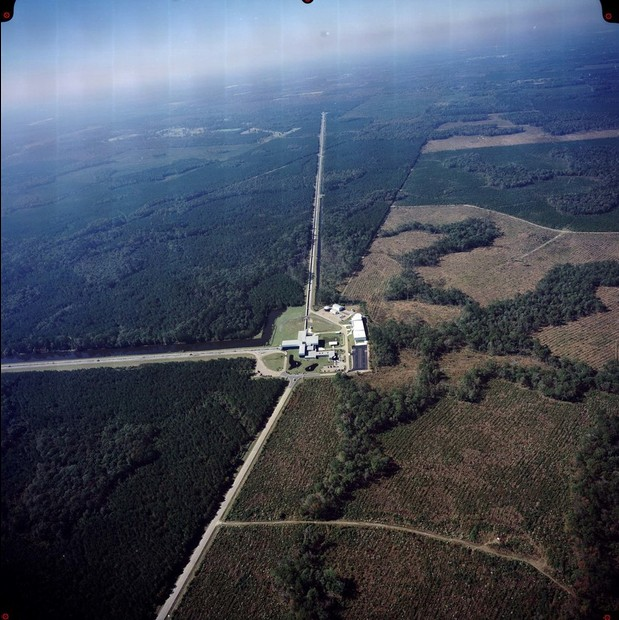
\includegraphics[width=2.5in]{LIGOLivingston.png}}
\hfil
\subfloat[]{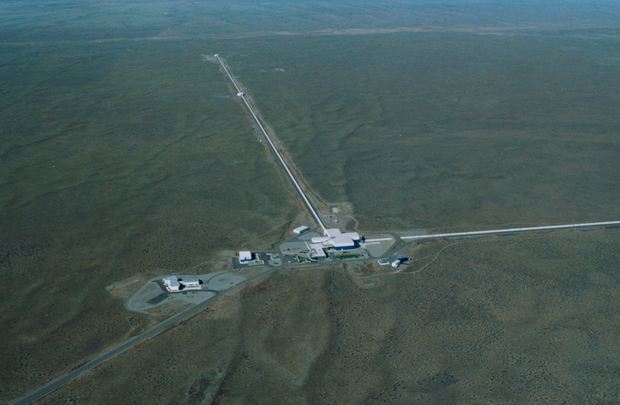
\includegraphics[width=2.5in]{LIGOHanford.png}}
\caption{Aerial pictures of LIGO.[3][4]}
\label{LIGO}
\end{figure*}

\begin{figure}[!t]
\centering
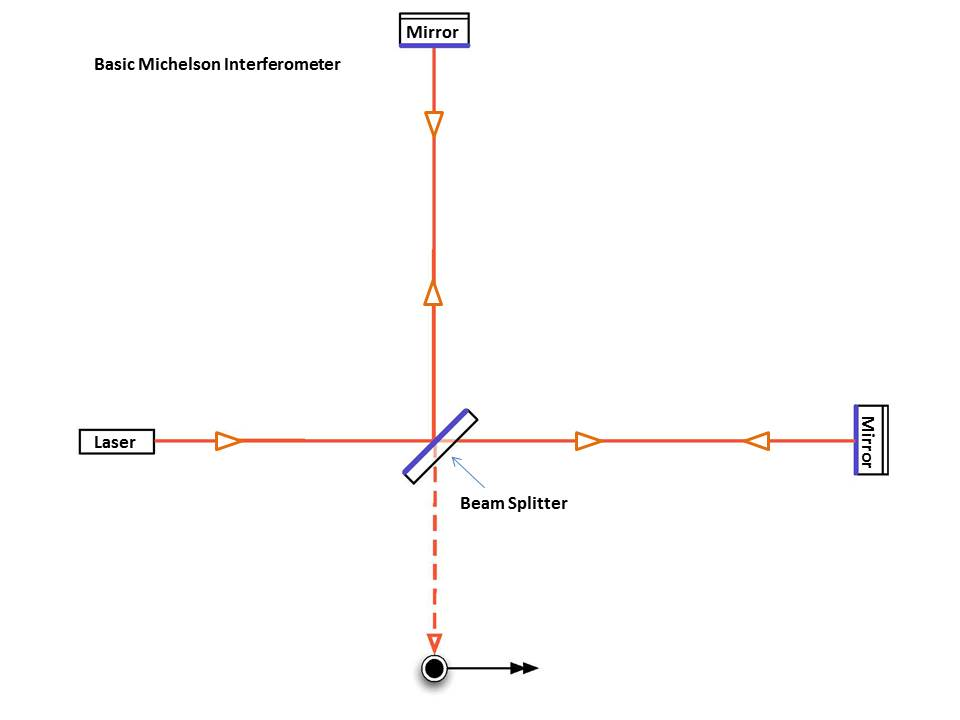
\includegraphics[width=2.5in]{interferometer.png}
\caption{Model of basic Michelson interferometer. The one ray of light is separated into two by the beam splitter and the two split ray of light merge again into one after two reflection and produce pattern of interference.[2]}
\label{interferometer}
\end{figure}

However, the LIGO's accuracy is $10^{-18}m$ which is a thousandth of the proton's scale[5]. The length of the arms of LIGO is still not long enough to make its accuracy to this order of magnitude if it is merely a basic Michelson Interferometer. Actually, in real LIGO project, a component called "Fabry Perot cavity" was installed between the mirrors and beam splitter as Fig. \ref{FabryPerot}. The light can be reflect back and forth for about 280 times from its entering Fabry Perot cavity to its leaving[5]. This component increases the sensitivity of LIGO dramatically and also saves the space occupied by LIGO.
\begin{figure}[!t]
\centering
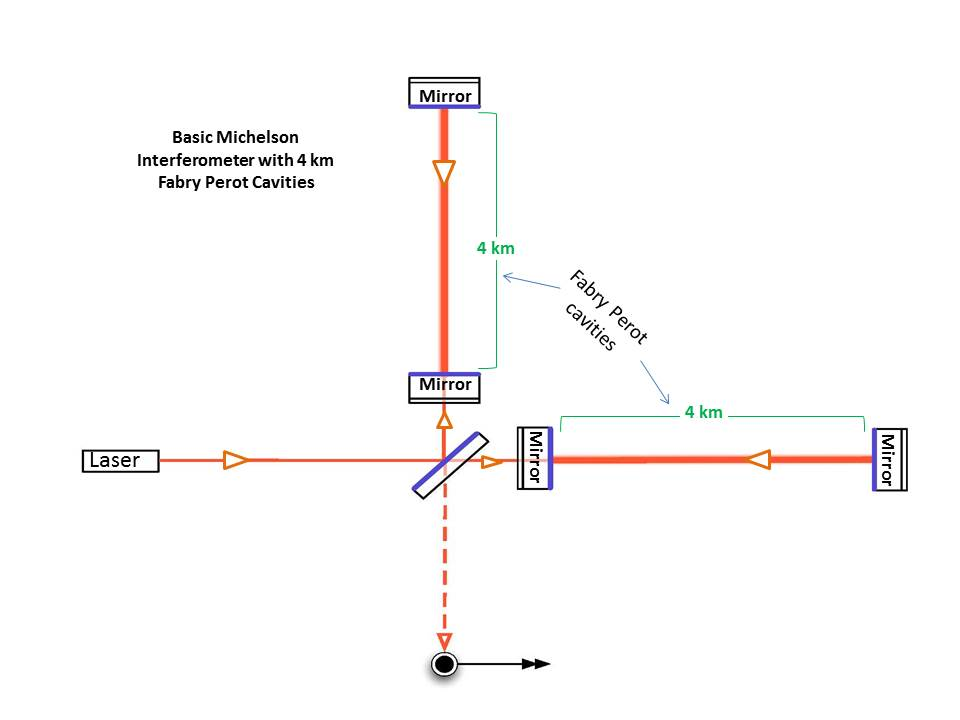
\includegraphics[width=2.5in]{FabryPerot.png}
\caption{Model of interferometer with Fabry Perot cavity. Fabry Perot cavity allows the light travel between the mirrors repeatedly and increases the distance that the light travels to make the device more sensitive.[6]}
\label{FabryPerot}
\end{figure}
\subsection{Power Boost Laser}
To improve the sensitivity of LIGO, the intensity of the laser also need enhancing to produce clearer pattern of interference. The theoretic value of the power LIGO need is 750 kilo Watts[5]. However, for LIGO working at full power, the laser produced and multi-amplified is still only 200 watts and it is technically difficult to increasing the intensity produced by LIGO[5]. To fix the problem, a "power recycling" mirror was installed between the source of laser and the beam splitter (Fig. \ref{PowerRecyclingMirror}), which is a kind of "one-way" mirror. It means that the light can go through it from its left side to its right side easily while almost all be reflected back when coming from the right side. In this way, the part of the laser that used to return to back (travel toward the source of the laser) can be reflect back and join the light entering, which realizes the function of recycling[5]. Therefore, the intensity of the light that finally comes to the photodetector will be much higher than it when produced by the source initially.

\begin{figure}[!t]
\centering
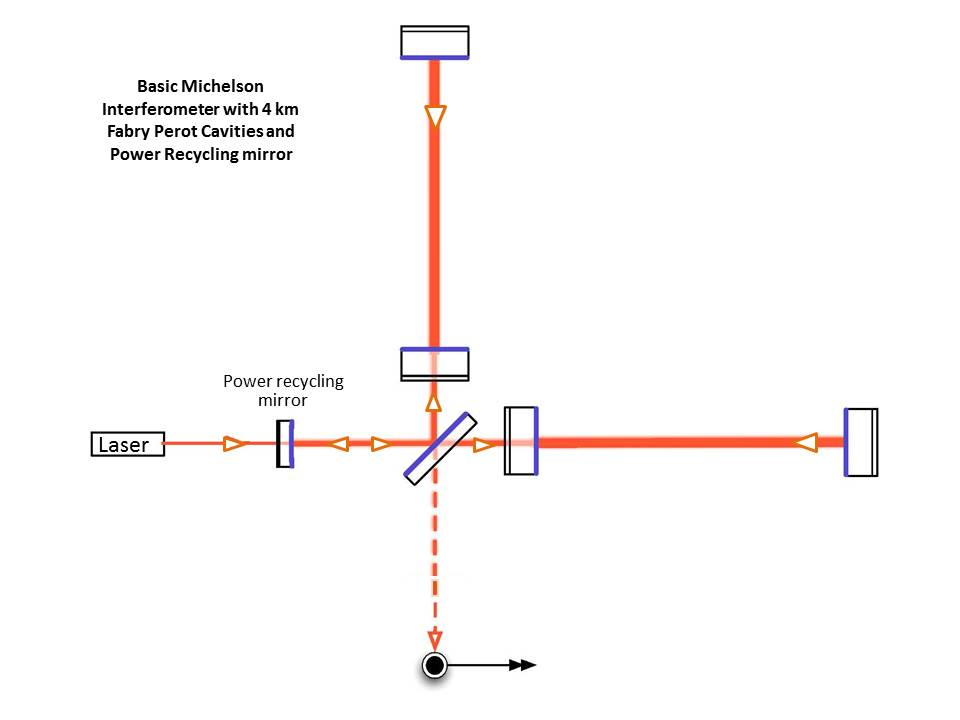
\includegraphics[width=2.5in]{PowerRecyclingMirror.png}
\caption{Model of interferometer with "power recycling" mirror. The "power recycling" mirror can enhance the intensity of the laser produced by LIGO to get clearer pattern of interference.[7]}
\label{PowerRecyclingMirror}
\end{figure}
\subsection{Seismic Isolation}
Because LIGO is so sensitive that any slight disturbance from the outside can affect the detection result. To overcome this potential disadvantage, the system that eliminates outside vibration is essential for LIGO to avoid noises to cover the the signal produced by the gravitational waves, which includes the positive damping system and passive damping system (Fig. \ref{Quad}), which work together to keep the components stable[9].

\begin{figure}[!t]
\centering
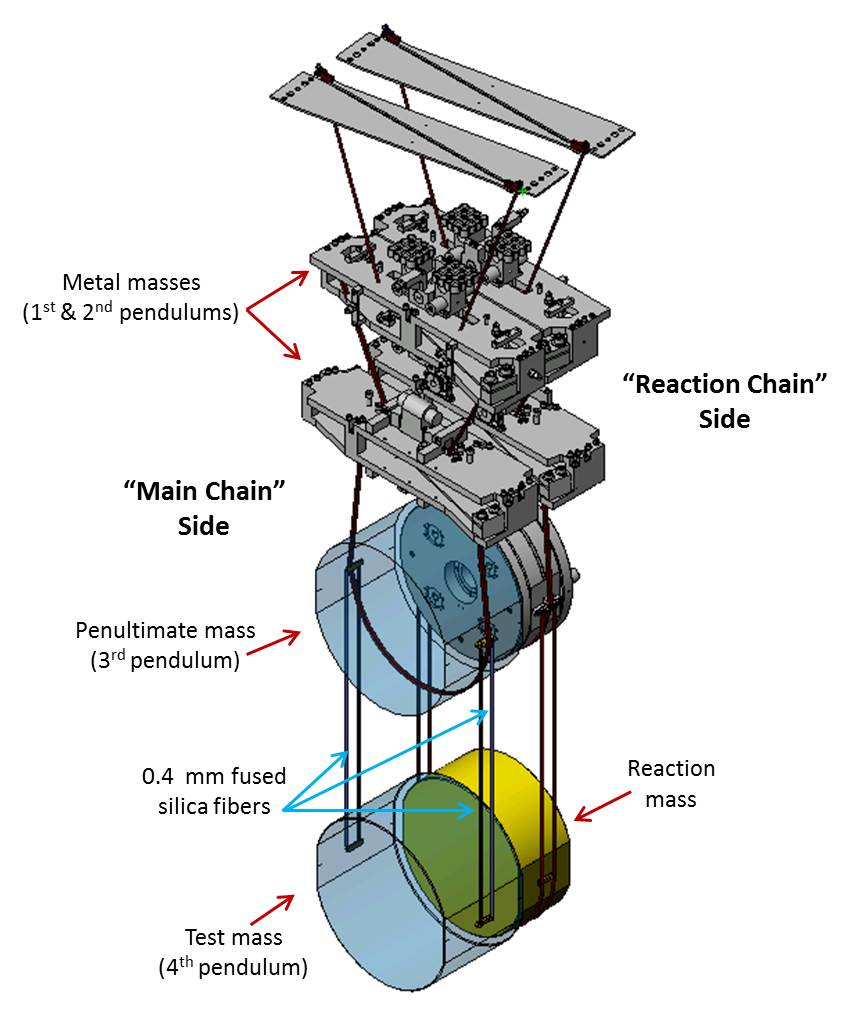
\includegraphics[width=2.5in]{Quad.png}
\caption{Passive damping system. The "Main Chain" side was faced with the rays of laser while the "Reaction Chain" side is responsible for keeping the mirror stable.[8]}
\label{Quad}
\end{figure}
\subsubsection{Active Damping System}
The Internal Seismic Isolation (ISI) system can sense the motion of the outside environment and perform inversely to keep the components of LIGO stable[9].
\subsubsection{Passive Damping System}
The passive damping system of LIGO suspends the mirrors with "quad", which is a 4-staged pendulum including four 0.4mm thick fused-silica fibers[9]. This passive damping system helps eliminate the noises further and the heavy wight (40 kilograms each) of the mirrors also restrains the vibration of the mirrors at the same time[9].
\subsection{Vacuum}
In order to avoid the air particles in Brownian movement to impact the mirrors irregularly and to affect the way that the laser ray travels to produce noises, all the components of LIGO system need placing in the nearly absolute vacuum. This strict condition is realized by the following measures. (1)Keep the tubes' temperature between $150 ^\circ C$ and $170 ^\circ C$ for a month to drive out the air; (2)Use Turbo-pump vacuums to pump out the air further; (3)Use the ion pump to first charge and then extract the single air molecules contained in the metal with electric field[9]. These measures enable the space inside LIGO reach the stage that the air pressure inside is only one-trillionth of it at sea level.
\subsection{Mirrors}
The high-intensitied laser requires high quality of the mirrors because slight absorption of the light by the mirrors can produce lots of heat during the about 280 reflection of the light in the Fabry Perot cavity, which will dramatically increase the temperature of the mirror, changing its physical properties and causing inaccuracy of the result and danger. Therefore, the mirrors of LIGO was made of very pure fused silica glass, which only absorb 1 photon out of $3\times{10}^6$ that meet the mirrors[9]. Furthermore, the mirrors are polished sophisticatedly to the order of magnitude of atom[9], which assures that the light will not travel out of its track during its about 280 reflection in Fabry Perot cavity.
\subsection{Dual Detector}
The LIGO was composed of two detectors, which are located in Livingston, Louisiana and Hanford Washington. The detector in different place are separated by 3002 kilometers. The reason to separate the two devices so far is that the impact of irrelevant vibrations on the earth like earthquake on the device at different place is different. Therefore, if the two devices get same or similar signals, conclusion can be derived that the signal was not cause by the irrelevant vibrations[10]. Furthermore, same or similar results from two devices at different places can be more convincible than it from one.
\section{The Revolution History Of LIGO}
\subsection{Weber bar}
Actually, LIGO is not the first device designed for the detection of gravitational waves. The first person that proposed idea and tried detecting gravitational waves is Joseph Weber, who invented a device called Weber bar as his tool[11]. At that time, Weber's Weber bar was mainly composed by two large aluminium bars suspended by thin lines, each of whose length measured 2 meters and diameter measured 1 meter. The quality factor of the two bar is very high, which means it cost very little energy when oscillating. Therefore, when gravitational waves passes the device, squeezing and stretching the space around, resonance can be generated, which will be amplified by piezoelectric sensors installed on the two bars to be the signal that can be detect. In1969, Weber claimed that the signal of gravitational wave was detected by his device[12]. However, his experiment result was found unable to be repeated by other research group and was seen as a mistake[16].

Although Weber bars had not produce any valid results and have flaws like inadequate accuracy and instability and its principle was different from today's LIGO, his efforts showed the possibility to detect gravitational waves and arose other researchers' interest in this field. The laser interferometer was invented by his student Robert Forward and his efforts for early try of detecting gravitational waves are universally acknowledged by the researchers who participated in the project of LIGO. One of the founder of LIGO, Kip S. Thorne, praised Weber as the "founding father of this field" after their news conference about their first detecting gravitational wave on February 11th, 2016[16].
\subsection{Early Theoretic Works and Construction of LIGO}
In 1962 two Soviet Physicists, Mikhail Gertsenshtein and Vladislav Pustovoit, formally proposed the idea of detecting gravitational waves using the interference of laser but did not conduct it[13]. Later in 1969, Rainer Weiss, who is specialized at laser, was inspired by a paper of Pirani Felix[14]. He could not understand Weber's experiment and had not heard the theoretic works accomplished by the two Russian Physicist at that time. Therefore, he designed a method of detecting gravitational waves with a interferometer on his own[15]. His idea was published on the internal periodical of Massachusetts Institute of Technology[15] but did not arose too much repercussions or convince many people. Later, he also made a real mini prototype which was 1.5 meter long using military fund, but was terminated before the device could work successfully[16].

Kip Thorne, who used to be suspicious of the method proposed by Weiss, reconsidered the method and was convinced of its feasibility after his communication with Weiss[16]. He persuaded California Institute of Technology to fund him with the project and invited Ronald Drever to help to create a lager prototype in 1983, whose length is 40 meters[16]. This project verified the feasibility of the interferometer whose length order of magnitudes is kilometer.

At that time, MIT and Caltech conducted their detection for gravitational waves separately. When the two group both applied fund from NSF (National Science Foundation), they had to merge their project under the pressure from NSF that refused to fund two large project with same aim[16].

The LIGO project suffered a period of difficult time because of conflict between the members and funding issue between 1984 and 1994 and made little progress on research[16]. This project was restarted in 1994 in Hanford, Waston State and 1995 in Livingston, Louisiana and roughly completed in 1997[16].

The initial LIGO (iLIGO) worked between 2002 and 2010[16]. However, it did not discover any signal of gravitational wave during its service because of its inadequate accuracy[16]. Even though, as a pathfinder, iLIGO developed basic technologies for LIGO. The LIGO device began its updating, which ended in 2015[16].
\subsection{Successful Observation}
From February, 2015, aLIGO (advanced LIGO) entered its "engineering mode" (test mode), and began its formal observation in September. It was not many days after its formal observation that LIGO first detected the signal of gravitational wave in human's history. The finding was verified carefully before the conference on February 11th, 2017[1], which testified Einstein's prediction in his General Theory of Relative and the feasibility of gravitational wave detection.

Till now, LIGO has detected gravitational wave of more five astronomical events, GW151226[17], GW170104[18], GW170608[19], GW170814[20] and GW170817[21], named after the date they were found.
\section{The Future Development Of LIGO}
\subsection{"A+"}
"A+" proposal provides a guideline for modest-cost upgrade on the base of aLIGO during 2017 and 2026. In "A+", squeezed light injection reduces the quantum noise, application of better coating with lower absorption rate reduces the thermal noise caused by the photon absorbed by the mirrors and the adoption of high stress fiber that used in quad can reduce suspension thermal noise by restrain the vibration of the mirrors[22]. According to theoretic estimation, these measures combined together can double the sensitivity of LIGO[23].
\subsection{LIGO Voyager}
LIGO voyager (LV) is another more important upgrade based on existing aLIGO, which is planned to come to use during 2027 and 2028[22]. LIGO voyager will also double sensitivity of original  LIGO and make its minimum frequency that can be detected half of its original value[22]. LV will apply a laser of higher energy (300-700W) and higher frequency (wavelength at 1550 nm) to reduce the scattering of the laser[22]. To neutralize the extra thermal noise and improve its sensitivity, LV is going to work in a temperature lower than $123K$. Besides, LV also will use the mirror with bigger weight (160 kilograms) to restrain noises caused by vibration[22].
\subsection{LIGO Cosmic Explorer}
LIGO cosmic explorer is a proposal for building a new observatory at a new place to detect the binary neutron star beyond one red-shift[22]. The proposal has not been mature yet. However, it is considered to have arms of much longer length (40kilometers) and work with other existing LIGO facilities[22].
\subsection{Scientific Plans And Facilities Of The Same Series As LIGO in Other Country}
There are also many facilities for gravitational wave detection in other countries. Some of them have cooperation with LIGO, like VIRGO and GEO600 in Europe while others are still under construction like KAGRA in Japan. China also raised its proposal of gravitational wave observatory called Taiji Plan and Tianqin Plan, which, however, are different from LIGO because it is not based on the ground but detects the gravitational waves with the facilities in the space. The space-based facility will avoid the noises from the ground and, therefore, more sensitive.[24][25] Facilities like LIGO can work together not just for reverifying Einstein's prediction for this mission has been generally completed by aLIGO but to develop a new method for astro-observation for human being because compared with the traditional observatory detecting electromagnetic wave, LIGO observes astronomy phenomena with gravitational wave. Besides, the cooperation and data sharing between the facilities can reduce the negative effect of noises on the results and make the results more convincible.
\section{Conclusion}
The development of LIGO and gravitational waves detection have gone through a long, difficult time and have improved its accuracy and stability with its repeated iteration. Through the first successful detection of gravitational wave, LIGO did not only verify Einstein's prediction in his General Theory of Relative but also introduced a brand new method for astronomical observation. That is, detecting the gravitational waves rather than the traditional way, detecting the electromagnetic waves. In the future, as the further updating of LIGO, the completion of similar facility and increasing of the corporation between the researchers of similar facilities, the accuracy of the detection of gravitational waves will be improved further and it will make possible for more specific data of gravitational waves detection, which may make gravitational detection one of the mainstream observation methods and promote people's knowledge about the space.





% if have a single appendix:
%\appendix[Proof of the Zonklar Equations]
% or
%\appendix  % for no appendix heading
% do not use \section anymore after \appendix, only \section*
% is possibly needed

% use appendices with more than one appendix
% then use \section to start each appendix
% you must declare a \section before using any
% \subsection or using \label (\appendices by itself
% starts a section numbered zero.)
%



% you can choose not to have a title for an appendix
% if you want by leaving the argument blank



% use section* for acknowledgment
\section*{Acknowledgment}


The author would like to thank everyone and everything.


% Can use something like this to put references on a page
% by themselves when using endfloat and the captionsoff option.
\ifCLASSOPTIONcaptionsoff
  \newpage
\fi



% trigger a \newpage just before the given reference
% number - used to balance the columns on the last page
% adjust value as needed - may need to be readjusted if
% the document is modified later
%\IEEEtriggeratref{8}
% The "triggered" command can be changed if desired:
%\IEEEtriggercmd{\enlargethispage{-5in}}

% references section

% can use a bibliography generated by BibTeX as a .bbl file
% BibTeX documentation can be easily obtained at:
% http://mirror.ctan.org/biblio/bibtex/contrib/doc/
% The IEEEtran BibTeX style support page is at:
% http://www.michaelshell.org/tex/ieeetran/bibtex/
%\bibliographystyle{IEEEtran}
% argument is your BibTeX string definitions and bibliography database(s)
%\bibliography{IEEEabrv,../bib/paper}
%
% <OR> manually copy in the resultant .bbl file
% set second argument of \begin to the number of references
% (used to reserve space for the reference number labels box)
\begin{thebibliography}{1}

\bibitem{IEEEhowto:kopka}
B.~P.~ Abbott et al., "Observation of gravitational waves from a binary black hole merger,"\emph{Physical Review Letters}, vol. 116, no. 6, p. 061102, Feb. 2016.

\bibitem{IEEEhowto:kopka}
LIGO Caltech, "Digital picture: A basic Michelson interferometer," \emph{LIGO Caltech}, 2016. [Online]. Available: https://www.ligo.caltech.edu/page/ligos-ifo. [Accessed: June. 16, 2018]

\bibitem{IEEEhowto:kopka}
LIGO Caltech, "Digital picture: LIGO's Livingston Louisiana detector," \emph{LIGO Caltech}, Dec. 3, 2009. [Online]. Availabe: https://www.ligo.caltech.edu/image/ligo20150731a. [Accessed: June. 16, 2018]

\bibitem{IEEEhowto:kopka}
LIGO Caltech, "Digital picture: An aerial Photo of LIGO's Hanford, Washington detector," \emph{LIGO Caltech}, May. 3, 2008. [Online]. Availabe: https://www.ligo.caltech.edu/image/ligo20150731e. [Accessed: June. 16, 2018]

\bibitem{IEEEhowto:kopka}
LIGO Caltech, "LIGO's interferometer," \emph{LIGO Caltech}, 2016. [Online]. Availabe: https://www.ligo.caltech.edu/page/ligos-ifo. [Accessed: June. 16, 2018]

\bibitem{IEEEhowto:kopka}
LIGO Caltech, "Digital picture: Basic Michelson interferometer with Fabry Perot cavities," \emph{LIGO Caltech}, 2016. [Online]. Availabe: https://www.ligo.caltech.edu/page/ligos-ifo. [Accessed: June. 16, 2018]

\bibitem{IEEEhowto:kopka}
LIGO Caltech, "Digital picture: Basic Michelson interferometer With Fabry Perot Cavities And Power Recycling Mirror," \emph{LIGO Caltech}, 2016. [Online]. Availabe: https://www.ligo.caltech.edu/page/ligos-ifo. [Accessed: June. 16, 2018]

\bibitem{IEEEhowto:kopka}
LIGO Caltech, "Digital picture: Anatomy of a quad," \emph{LIGO Caltech}, 2016. [Online]. Availabe: https://www.ligo.caltech.edu/page/ligo-technology. [Accessed: June. 16, 2018]

\bibitem{IEEEhowto:kopka}
LIGO Caltech, "LIGO technology," \emph{LIGO Caltech}, 2016. [Online]. Availabe: https://www.ligo.caltech.edu/page/ligo-technology. [Accessed: June. 16, 2018]

\bibitem{IEEEhowto:kopka}
LIGO Caltech, "LIGO's dual detectors," \emph{LIGO Caltech}, 2016. [Online]. Availabe: https://www.ligo.caltech.edu/page/ligo-detectors. [Accessed: June. 16, 2018]

\bibitem{IEEEhowto:kopka}
J.~Weber, "Detection and generation of gravitational waves,"\emph{Physical Review}, vol. 117, no. 117, p 306, 1960.

\bibitem{IEEEhowto:kopka}
J.~Weber, "Evidence for discovery of gravitational radiation,"\emph{Physical Review Letters}, vol. 22, no. 24, pp. 1320-1324, June. 16, 1969.

\bibitem{IEEEhowto:kopka}
M.~E.~Gertsenshtein, "Wave resonance of light and gravitional waves,"\emph{Sov Phys JETP}, vol. 14, pp. 84-85, 1962.

\bibitem{IEEEhowto:kopka}
F.~A.~E.~Pirani, "Republication of: On the physical significance of the Riemann tensor,"\emph{General Relativity and Gravitation}, vol. 41, no. 5, pp. 1215-1232, 2009.

\bibitem{IEEEhowto:kopka}
R.~Weiss, "Electromagnetically coupled broadband gravitational antenna,"\emph{Quarterly Progress Report 105}, 1972.

\bibitem{IEEEhowto:kopka}
J.~L.~Cervantes-Cota, S.~Galindo-Uribarri, and G.~F.~Smoot, "A brief history of gravitational waves,"\emph{Universe}, vol. 2, no. 3, p. 22, 2016.

\bibitem{IEEEhowto:kopka}
B.~P.~Abbott et al., "GW151226: observation of gravitational waves from a 22-solar-mass binary black hole coalescence,"\emph{Physics Review Letters}, vol. 116, p. 241103, 2016.

\bibitem{IEEEhowto:kopka}
B.~P.~Abbott et al., "GW170104: observation of a 50-solar-mass binary black hole coalescence at redshift 0.2,"\emph{Physics Review Letters}, vol. 118, no. 22, p. 221101, 2017.

\bibitem{IEEEhowto:kopka}
B.~P.~Abbott et al., "GW170608: Observation of a 19 solar-mass binary black hole coalescence,"\emph{The Astrophysical Journal Letters}, vol. 851, no. 2, p. L32, 2017.

\bibitem{IEEEhowto:kopka}
B.~P.~Abbott et al., "GW170814: A three-detector observation of gravitational waves from a binary black hole coalescence,"\emph{Physics Review Letters}, vol. 119, no. 14, p. 141101, 2017.

\bibitem{IEEEhowto:kopka}
B.~P.~Abbott et al., "GW170817: observation of gravitational waves from a binary neutron star inspiral,"\emph{Physics Review Letters}, vol. 119, no. 16, p. 161101, 2017.

\bibitem{IEEEhowto:kopka}
LIGO Scientific Collaboration, "Instrument Science White Paper,"\emph{LIGO Scientific Collaboration}, 2016. [Online]. Available: https://dcc.ligo.org/public/0120/T1500290/003/T1500290.pdf.

\bibitem{IEEEhowto:kopka}
J.~Miller et al., "Prospects for doubling the range of Advanced LIGO,"\emph{Physics Review D}, vol. 91, no. 6, p. 062005, 2015.

\bibitem{IEEEhowto:kopka}
Z.~Liu, Y.~Piao, and C.~Qiao, "Multi-band Gravitational Wave Universe Research and Space Taiji Project,"\emph{Mordern Physics Knowledge}, vol. 5, p. 007, 2016.

\bibitem{IEEEhowto:kopka}
Z.~Liu, "'The Tianqin Plan' captures the universe in space,"\emph{Technology Review}, vol. 43, no. 3, pp. 53-54, 2016.

\end{thebibliography}

% biography section
%
% If you have an EPS/PDF photo (graphicx package needed) extra braces are
% needed around the contents of the optional argument to biography to prevent
% the LaTeX parser from getting confused when it sees the complicated
% \includegraphics command within an optional argument. (You could create
% your own custom macro containing the \includegraphics command to make things
% simpler here.)
%\begin{IEEEbiography}[{\includegraphics[width=1in,height=1.25in,clip,keepaspectratio]{mshell}}]{Michael Shell}
% or if you just want to reserve a space for a photo:

% if you will not have a photo at all:
\begin{IEEEbiographynophoto}{Jialin Chen}
was born in Zhejiang Province, People Republic of China, in 1999. He is going to receive B.S. degree in physics from ShanghaiTech University in 2021.
\end{IEEEbiographynophoto}

% insert where needed to balance the two columns on the last page with
% biographies
%\newpage

% You can push biographies down or up by placing
% a \vfill before or after them. The appropriate
% use of \vfill depends on what kind of text is
% on the last page and whether or not the columns
% are being equalized.

%\vfill

% Can be used to pull up biographies so that the bottom of the last one
% is flush with the other column.
%\enlargethispage{-5in}



% that's all folks
\end{document}


